After I analyzed the impact on data rate and robustness of the physical layer parameter, I will simulate a platooning scenario in ns-3 to find the influence of the physical layer configuration on the network performance.


The network performance metric consists of the transmission latency, which describes the time needed to transmit the data
on the application layer, and the update rate of the platooning service, which defines how long ago a new position update
was received by the \ac{TM} in the Platooning Service.

Ns-3 is suitable for this simulation because it supports application layer-level simulation.
Via the extension Netsimulyzer, a graphical user interface is available to visualize the simulation results.

Any packets in ns-3 can be tagged with a packet Tag \footnote{\url{https://www.nsnam.org/docs/release/3.36/doxygen/classns3_1_1_tag.html}},
which are designed to add additional information to the packet.
Every added packet Tag belongs to the packet and does not change the packet size or characteristics.
Throughout the simulation, I used packet tags to add information that needed to be transferred.

The simulation scenario is based on the corn harvest and loading scenario, which is described in \autoref{sec:corn_harvest_scenario}, where
multiple \ac{FH}s harvest the corn and load it onto one of the \ac{TM}s.

Thereby, every \ac{FH} starts in the lower left corner of the field and harvests the corn along the path,
which is displayed in \autoref{fig:PlatooningRoute}.
As soon as a \ac{FH} reaches a field border, it makes a U-turn and continues
in the opposite direction.
Every \ac{FH} harvests the corn until it reaches the end of the field in the lower right corner.
The initial position of the \ac{TM}s is a row below the \ac{FH}s, which is displayed in \autoref{fig:PlatooningInit}.
\begin{figure}[H]%
   \centering
   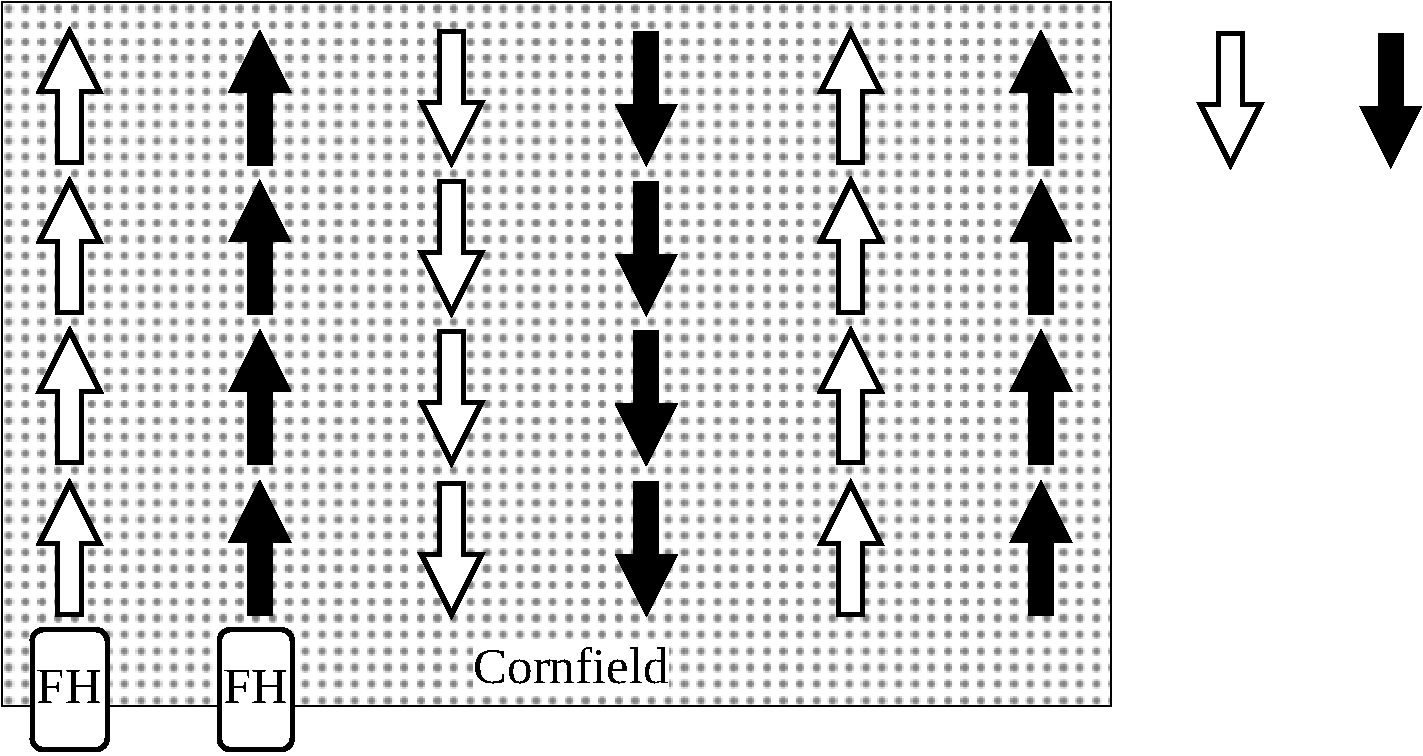
\includegraphics[width=0.7\textwidth]{figures/drawings-Route}
   \caption{Path of the \acf{FH} for harvesting corn on the field}
   \label{fig:PlatooningRoute}%
\end{figure}

An ns-3 Node represents every machine.
Each Node has a mobility model, which describes the movement of the machine.
In order to exchange data between the machines, every machine is equipped with an  ns-3 IEEE 802.11ax WifiNetDevice.
Every Wi-Fi Device runs in Ad-Hoc mode to enable direct communication
between the machines.
The Wi-Fi data rate is managed by a Constant Rate Wi-Fi Manager, which has a Non-Uniform
transmission mode and a data mode for uniform transmissions.
The transmission modes are configured according
to the parameters in \autoref{tab:SimulationParametersWiFi}.

The parameters are chosen from the results of the physical layer analysis of \autoref{sec:DataRate} and \autoref{sec:Robustness}.
Non-uniform transmissions are used to broadcast the Agricultural Platooning Service advertisements.

The non-uniform transmission parameters enable the longest possible
transmission range, which results in the lowest data rate.
Since no high data rate is required to advertise the Service, I chose the parameters to maximize the transmission range.
Uniform transmission parameters exchange Agricultural Platooning Service data between
the \ac{FH} and the \ac{TM}. \todo{Robustness?DataRate? Fieldexperiments}

Guidance data in the Agricultural Platooning Service is exchanged between the \ac{FH} and the \ac{TM} via the
uniform transmission mode.
The process data in \autoref{chap:cornHarvestData} reflects that a short transmission range
is sufficient to exchange the guidance data, which must still be robust against multipath effects.
I chose the parameters to balance a high robustness and high data rate.

The simulation is based on the ns-3 ConstantSpeedPropagationDelayModel and the  ns-3 FriisPropagationLossModel,
which represents signal propagation in free space.
\todo[color=yellow]{explain?}

\begin{table}[H]
	\centering
	\begin{tabular}{p{6cm}p{4cm}}
		General Parameters & \\
		\midrule
		Wi-Fi Standard & IEEE 802.11ax\\
		\ac{GI} & \SI{3200}{\nano\second}\\
		Frequency Spectrum & \SI{5.6}{\giga\hertz}\\
		\ac{BW} & \SI{20}{\mega\hertz}\\
		Max. Transmission Power & \SI{25}{\decibel}\\
		Antenna Gain & \SI{5}{\dB}\\
		Maximum retries & \num{3}\\
		 & \\
		Uniform Transmission Parameters & \\
		\midrule
		\ac{MCS} & \num{5}\\
		Number \ac{MIMO} Streams & \num{2}\\
		 & \\
		Non-Uniform Transmission Parameters & \\
		\midrule
		Broadcast \ac{MCS} & \num{0}\\
		\ac{ER} mode enabled & True\\
		\ac{DCM} enabled & True\\
	\end{tabular}
	\caption{Simulation parameters for Wi-Fi Devices}
	\label{tab:SimulationParametersWiFi}
\end{table}

Every machine node runs an ns-3 Application responsible for the Agricultural Platooning Service.
The application is identified by a unique identifier and runs a UDP socket to exchange data with other Agricultural Platooning Service applications.
Every UDP socket can be addressed by an IP address and a port number.
The IP address is the IP address of the machine node.

In the beginning, every \ac{FH} broadcasts a search request $search\_TM$ via the non-uniform transmission mode to find an empty \ac{TM} to load the corn onto according to
to the procedure in \autoref{alg:SearchTM}.
As shown in \autoref{fig:PlatooningInit}, multiple \ac{TM}s receive the search request and answer with
their current fill level of the \ac{TM}'s trailer.
The \ac{FH} chooses the \ac{TM} with the lowest fill level and sends a connection request to the \ac{TM}.
As soon as the \ac{TM} receives the connection request, it answers with a connection response.
When the \ac{FH} receives the connection response, the Agricultural Platooning Service is started.
When no \ac{TM} answers the search request, the \ac{FH} repeats the search request every $search\_TM\_interval$ seconds.
\begin{figure}[H]%
   \centering
   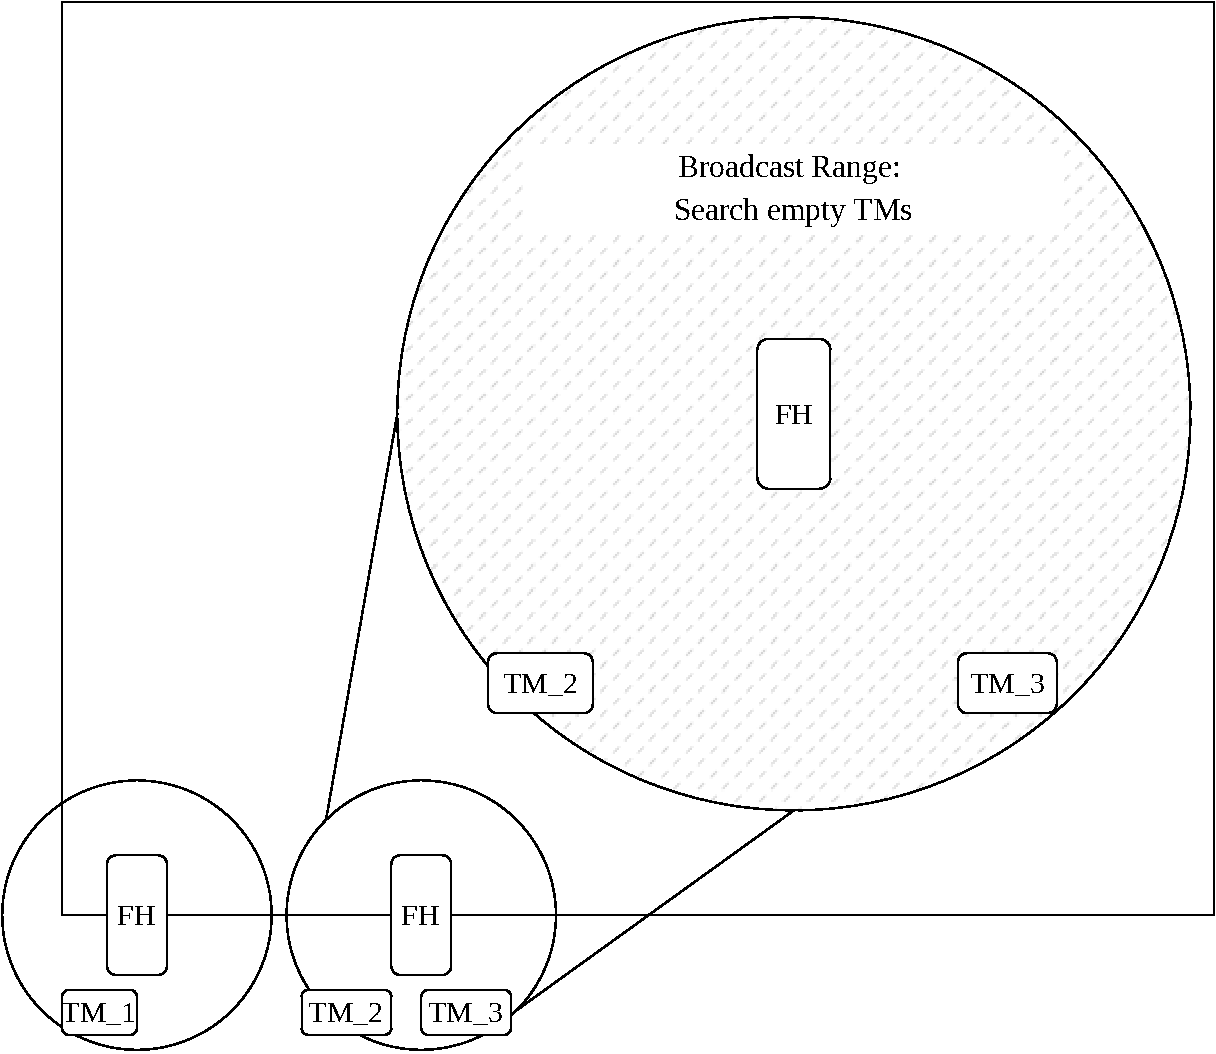
\includegraphics[width=0.7\textwidth]{figures/platoonINIT}
   \caption{Start position of the \acf{FH}s and \acf{TM}s, where a \ac{FH} broadcasts a search request to find
   a \ac{TM} to load the corn onto}
   \label{fig:PlatooningInit}%
\end{figure}

\begin{algorithm}
\begin{algorithmic}[1]
\REQUIRE Defined $search\_TM\_interval$, $search\_TM\_packet\_length$
\STATE Create packet $search\_TM$ of length $search\_TM\_packet\_length$ bytes
\STATE Broadcast $search\_TM$ to all \acs{TM}s
\IF {no \acs{TM} ansers}
    \STATE Repeat Broadcasting $search\_TM$ every $search\_TM\_interval$ seconds
\ELSE
   \STATE Send connection request
   \IF {No \acs{TM} response}
      \STATE Repeat Broadcasting $search\_TM$ every $search\_TM\_interval$ seconds
   \ELSE
      \STATE Connection established
      \STATE Start Agricultural Platooning Service
   \ENDIF
\ENDIF
\end{algorithmic}
\caption{Procedure of the \acf{FH} to search for a \acf{TM} to load the corn onto}
\label{alg:SearchTM}
\end{algorithm}

Next, the \ac{FH} starts to harvest the corn.
All steps of the harvest process and Agricultural Platooning Service are summarized in
\autoref{alg:UpdateTM}.

\begin{algorithm}
\begin{algorithmic}[1]
\REQUIRE Defined $platoon\_data\_interval$, $platoon\_data\_packet\_length$
\STATE Calculate harvested volume
\STATE Advance \ac{FH} position
\STATE Add harvested volume to \ac{TM} fill level
\IF {\ac{TM} fill level is full}
    \STATE Disconnect from current \ac{TM}
	\STATE Start Agricultural Platooning Service with waiting \ac{TM}
\ELSE
	\STATE Create packet $TM\_data$ of length $platoon\_data\_packet\_length$ bytes, which contains the \ac{TM} fill level and the new guidance position
	\STATE Send $TM\_data$ to \ac{TM}
	\IF {\ac{TM} fill level is half full}
		\STATE Start \autoref{alg:SearchTM} to search for new \ac{TM}
	\ENDIF
\ENDIF
\end{algorithmic}
\caption{Procedure of the \acf{FH} to send the \acf{TM} fill level and the \ac{TM} guidance position every
\textit{platoon\_data\_interval}}.
\label{alg:UpdateTM}
\end{algorithm}

The FH harvest process is defined by the harvest states in \autoref{tab:HarvestStates},
where every harvest state represents a different \ac{PD} and \ac{FH} speed.
When the \ac{PD} is low, the \ac{FH} can harvest faster and vice versa.

Starting in the harvest state H1, the \ac{FH} determines the next harvest state every \SI{50}{\milli\second}
by the Markov chain in \autoref{fig:MarkovChain}.
This Markov chain ensures that the harvest state can't transverse from H0 to H2 directly, which would represent
a low \ac{PD} immediately followed by a high \ac{PD}.
As I do not have enough harvest process data, which contain the \ac{PD} and the \ac{FH} speed,
I chose the transition probabilities to the best of my knowledge.\todo[color=yellow]{by common sense?}.

\begin{table}[H]
	\centering
	\begin{tabular}{>{\centering}p{2cm}p{4cm}p{4cm}}
		\toprule
		Harvest State & \ac{PD} & \ac{FH} speed\\
		\midrule
		H0 & \SI{30}{\tonne\per\hectare}
        & \SI{10}{\kilo\metre\per\hour} \\
		H1 & \SI{40}{\tonne\per\hectare}
        & \SI{8}{\kilo\metre\per\hour} \\
		H2 & \SI{50}{\tonne\per\hectare}
        & \SI{6}{\kilo\metre\per\hour} \\
		\bottomrule
	\end{tabular}
	\caption{Corn harvest states, which define a range of \acf{PD}s and \acf{FH} speeds, where the data is based on the
	key figures \cite{faustzahlen2018}}
	\label{tab:markov_chain}
\end{table}

\begin{figure}[H]
\centering
\begin{tikzpicture}[->, >=stealth', auto, semithick, node distance=3cm]
	\tikzstyle{every state}=[fill=white,draw=black,thick,text=black,scale=1]
    \node[circle, draw]    (A)               {H0};
	\node[circle, draw]    (B)[right of=A]   {H1};
	\node[circle, draw]    (C)[right of=B]   {H2};
	\path
	(A) edge[loop left]			node{0.7}	(A)
        edge[bend left,above]	node{0.3}	(B)
	(B) edge[bend left,below]	node{0.2}	(A)
        edge[bend left,above]   node{0.2}	(C)
        edge[loop]		        node{0.6}	(B)
	(C) edge[bend left,below]	node{0.3}	(B)
        edge[loop right]		node{0.7}	(C);
	\end{tikzpicture}
\caption{Markov Chain for the states \acf{PD} 0, 1 and 2, which represent the current \ac{PD} and
harvest speed from \autoref{tab:markov_chain}.}
\label{fig:MarkovChain}
\end{figure}

After determining the next harvest state, the \ac{FH} sets the \ac{PD} and the \ac{FH} speed according to the defined values in
\autoref{tab:HarvestStates}.
The position of the \ac{FH} is advanced by the \ac{FH} speed multiplied with \SI{50}{\milli\second} along the
harvest path in \autoref{fig:PlatooningRoute}.
The harvested volume during this $platoon\_data\_interval$ is calculated with the following
equations:
\begin{equation}
   \label{eq:AreaCalculation}
   \text{Harvested Area} =
      \text{Harvest width} \times \text{Harvest speed} \times \text{Time step}
   ,
\end{equation}
\begin{equation}
   \label{eq:VolumneCalculation}
   \text{Harvested Volumne} =
   \text{Harvested Area} \times \text{\ac{PD}} \times \text{Corn volume per tonne}.
\end{equation}

The harvested area is represented in \si{\hectare}, and
the harvested volume is defined in \si{\cubic\metre}.
The needed parameters for the calculation are from \cite{faustzahlen2018} and are listed in \autoref{tab:SimulationParameters}.
The calculated harvested volume is added to the \ac{TM}'s fill level, which is tracked by the \ac{FH}'s application.
Keeping track of the fill level represents the knowledge of the \ac{FH} about the \ac{TM}'s fill level, which the \ac{FH} would
normally get through a sprout guidance system.

Next, the \ac{FH} determines whether the \ac{TM} is full.
If the \ac{TM} is full, the \ac{FH} stops harvesting and sends a disconnect request to the \ac{TM}.
The \ac{TM} answers with a disconnect response and leaves the field to unload the corn.

If the \ac{TM} is not full, the \ac{FH} sends the $TM\_data$ to the \ac{TM},
which contains the new \ac{TM} fill level and the new guidance position.
The \ac{TM} updates the fill level and drives to the new position to load the corn, as shown in \autoref{fig:PlatooningHF}.
The guidance data positions the \ac{TM} always \SI{5}{\metre} left of the \ac{FH} because this part of the field was already harvested.
The distance between the \ac{FH} and the \ac{TM} is  as the \ac{FH} and the \ac{TM} moved mostly with a distance of around \SI{5}{\metre} in
the recorded process data in \autoref{chap:cornHarvestData}.

If the \ac{TM} fill level is half full, the \ac{FH} starts the \autoref{alg:SearchTM}
to search for a new \ac{TM} to load the corn onto.
This process is visualized in \autoref{fig:PlatooningHF}.
As soon as the \ac{FH} finds a new \ac{TM}, the \ac{FH} connects to the new \ac{TM} and starts sending
the \ac{TM} guidance positions, which place the \ac{TM} \SI{12}{\metre} behind the \ac{FH}.
The \ac{FH} continues harvesting until the \ac{TM} is fully loaded.
Meanwhile, the new \ac{TM} is waiting behind the \ac{FH} and can take over the loading position next to the \ac{FH} as
soon as the \ac{TM}, where the \ac{FH} is currently loading onto, is full.

A fully loaded \ac{TM} leaves the field to unload the corn and returns to the position where it disconnected from the \ac{FH}.
There, it waits for an incoming "search\_TM" request from a \ac{FH} to connect to a \ac{FH} again.

The corn harvest process is finished when the last \ac{FH} has finished harvesting and moved to the end of the field as
shown in \autoref{fig:PlatooningRoute}.

Each corn harvest scenario is visualized to ensure the correctness of the simulation.

Every simulation configuration runs \num{5} times, where every \ac{FH} harvests \SI{1}{\hectare} of corn, which equals to roughly
\num{2.5} \ac{TM} loads.

\begin{table}[H]
	\centering
	\begin{tabular}{p{5cm}p{4cm}}
		\toprule
		Parameters & \\
		\midrule
		\textit{search\_TM\_interval} & \SI{1}{\second}\\
		\textit{search\_TM\_packet\_length} & \SI{0.5}{\kilo\byte}\\
		\textit{platoon\_data\_interval} & \SI{50}{\milli\second}\\
		\textit{platoon\_data\_packet\_length} & \SI{1}{\kilo\byte}\\
		Platoon Overloading Distance & \SI{5}{\meter}\\
		Field Size & \SI{2000}{\meter} x \SI{1000}{\meter}\\
		\bottomrule
	\end{tabular}
	\caption{Simulation parameters for the Application Agricultural Platooning Service}
	\label{tab:SimulationParameters}
\end{table}



\textcite{zhang_method_2009} defined a data frame of \SI{32}{\byte}, which includes an identifier, timestamp, longitude,
latitude, heading, speed and direction.
This set of data comprises a basic set which can be sufficient for the implementation of a platooning service,
as the authors show.
\textcite{schlingmann_aef_2019} do not specify the amount of data further and point out that the required data rate
for platooning services is low.

I have set the data size \textit{platoon\_data\_packet\_length} to \SI{1}{\kilo\byte} for the simulation of platooning services.
This data size is an abstraction of the storage space that may be needed for additional data or implementations
of authentication and security mechanisms.
In the Corn Harvest scenario, additional data could be, for example, the fill level of the transport machine.



Service Discovery

Rebroadcast by Count?
additional Traffic

MANET Service discovery

Visualisierung Netsimulyzer

Farbcodes

\begin{figure}[H]%
	\centering
	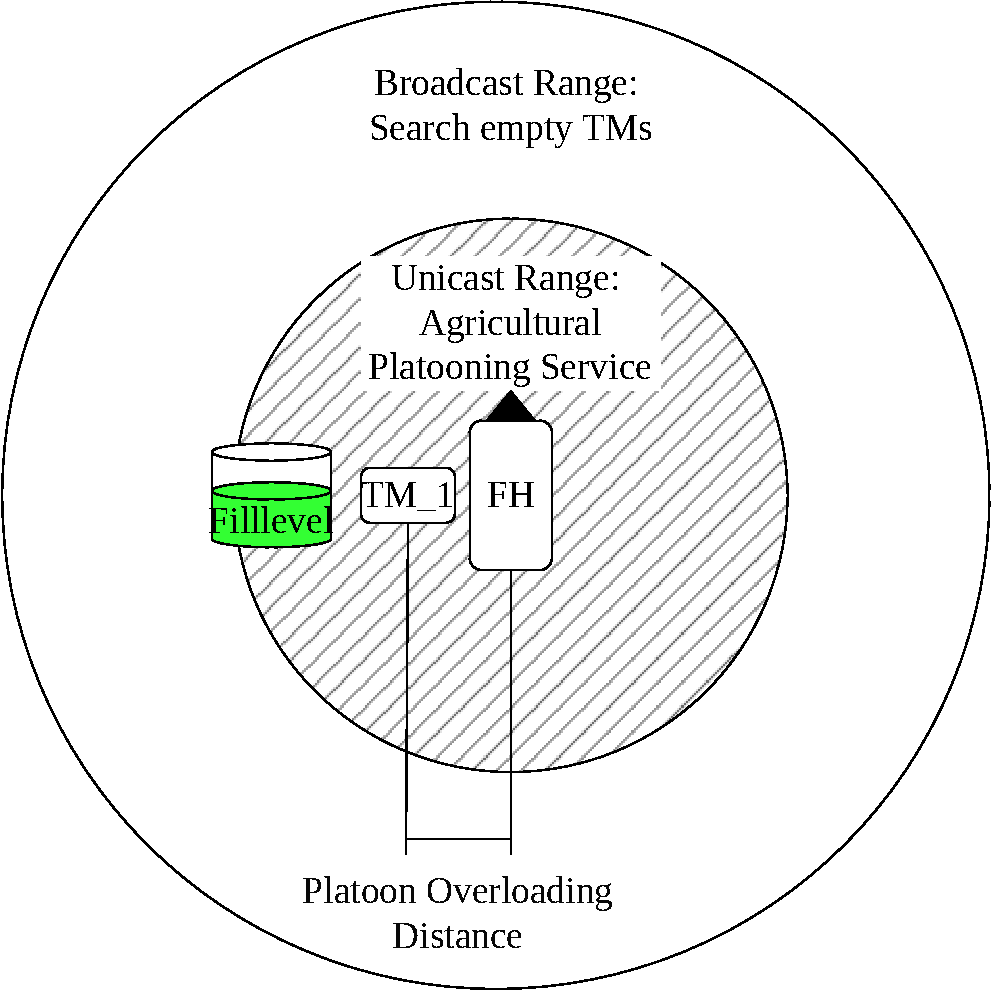
\includegraphics[width=0.7\textwidth]{figures/platoonHALF}
	\caption{\acf{TM} position left of the \acf{FH} for overloading, where the \ac{TM} is half full and the
		\ac{FH} starts the \autoref{alg:SearchTM} to search for a next empty \ac{TM},
		which can later take over the loading position.}
	\label{fig:PlatooningHF}%
\end{figure}

\begin{figure}[H]%
	\centering
	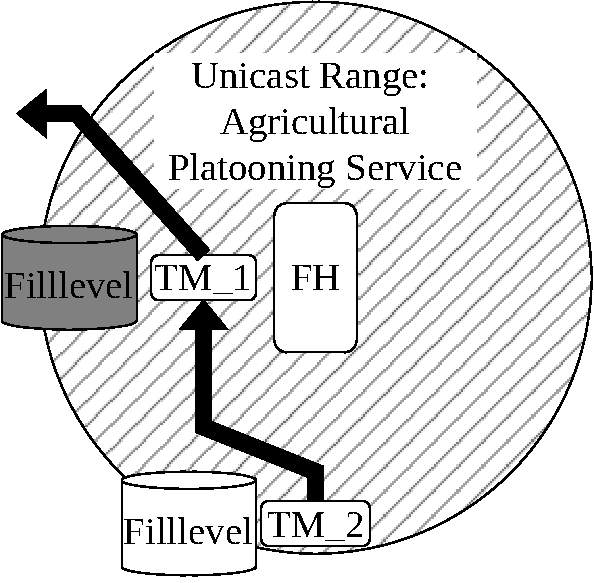
\includegraphics[width=0.5\textwidth]{figures/platoonFULL}
	\caption{Change of \acf{TM}s in the Application Agricultural Platooning Service, where $TM\_1$
	is full and leaves the field while the empty $TM\_2$ takes over the overloading position.}
	\label{fig:PlatooningFull}%
\end{figure}

\begin{figure}[]%
	\centering
	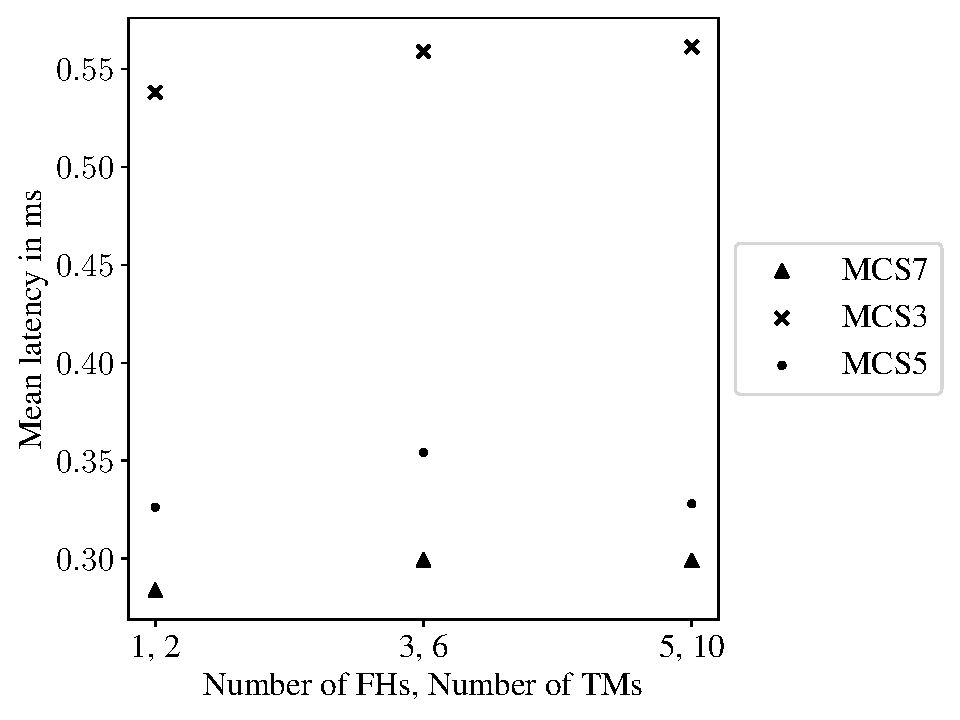
\includegraphics[width=0.8\textwidth]{figures/mean_scatter_2latency}
	\caption{Mean latency of the Application Agricultural Platooning Service in regards to the number of \ac{FH}s and \ac{TM}s and
	the chosen \ac{HE}-\ac{MCS} value.}
	\label{fig:mean_latency}%
\end{figure}
\begin{figure}[]%
	\centering
	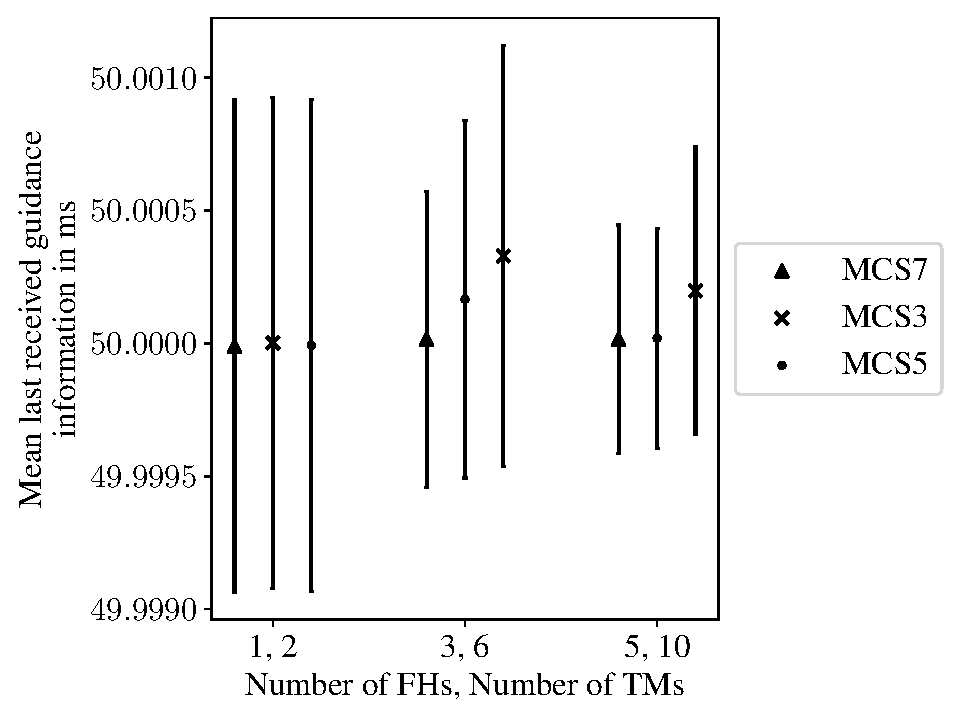
\includegraphics[width=0.8\textwidth]{figures/mean_scatter_2lastUpdate}
	\caption{Mean last guidance update of the Application Agricultural Platooning Service in regards to the number of \ac{FH}s and \ac{TM}s and
	the chosen \ac{HE}-\ac{MCS} value.}
	\label{fig:mean_lastUpdate}%
\end{figure}

